\chapter{Validation}
\section{implémentation}
expliquer comment on a fait pour implémenter. Quel était les moyen mis en place pour faire un bon logiciel.

schéma uml

comcomber

rspec

factories

metrics (travis, gemnasium, codeclimate, coveralls, railsbestpractice)

\section{Expériences}
Cette section aborde les expériences réalisées pour ce travail. Ceci commence par une après midi chez kidscode en petit groupe avec des initiés, vient ensuite le printemps des sciences pendant lequel environ 80 élèves ont tester l'application. Enfin, vient une analyse des expérience à travers des formulaires remplis par les élèves et les professeurs.
\subsection{kidscode}
\label{kidscode}
Dans le cadre de ce mémoire plusieurs expériences ont été menées. La première s'est déroulée chez Kidscode. Cette organisation a été présentée dans la section \ref{init-kidscode}. C'est une petit initiative locale qui apprend la programmation à 10 enfants âgé de 10 a 14 ans.

\subsubsection{Contexte}
\label{context-kidscode}
Il est important de définir le contexte et le publique de l'expérience car il peut avoir une influence considérable sur l'analyse de l'expérience.\\

Lors de cette expérience le publique était composé de 10 enfant de 10 à 14 ans ayant déjà fait une demi année de programmation dans le cadre du projet Kidscode. Le niveau de ces enfants n'est donc pas à négliger. Ils sont habitués à exécuter un programme et maîtrisent les principaux concepts de la programmation.\\

\subsubsection{Buts}
Le but poursuivit dans cette expérience est de valider l'utilisabilité de la plateforme et également le niveau de difficulté des missions proposées. Un autre but était de se familiariser avec le public en petit groupe, en préparation de la seconde expérience.

Ce dernier point pourrait sembler être moins justifié dans le cadre d'un mémoire sur l'informatique, mais la manière d'aborder les enfants est tout aussi importante que la qualité de l'application. Pour limiter le plus possible les biais dus à un manque de pédagogie ou d'expérience dans la gestion d'un groupe d'enfant, il était important de pouvoir avoir cette première expérience.
\subsubsection{Déroulement}
L'expérience s'est déroulée pendant un peu plus d'une heure. Les enfants avaient dans les premières heures l'activité habituelle de kidscode et la dernière heure était dédiée à l'expérience. 

Comme le changement d'activité était clairement annoncé, le début de l'expérience fut marqué par beaucoup de pertes d'attention et de dissipations. Un fois le groupe repris en main, les jeunes ont directement montré beaucoup intérêt. Pour l'interface qu'ils découvraient qui semblait leur plaire, tout comme pour la compétition intergroupe qui s'est rapidement mis en place.\\

Comme expliqué dans la partie précédente \ref{context-kidscode}, le public avait déjà de bonne notion de programmation par rapport au publique visé par ce mémoire. Les premières missions sont donc passées très vite. Les seuls points de ralentissement étaient principalement des problèmes de lecture des consignes. 

A ce moment, les consignes étaient toutes uniquement écrites. Cela a posé un problème car les jeunes ne prenaient pas le temps de les lire et donc ne savaient pas quoi faire. Ceci malgré la possibilité de retrouver les consigne via les menus de l'application. Ce manque d'intérêt pour les consignes ne venait pas d'un problème de niveau de lecture mais simplement d'une impatience face à l'expérience ce qui peut s'expliquer par le manque de rigueur dû à leur âge.\\

La compétition que les jeunes ont mis en place dès le début a eu un effet bénéfique pour leur évolution car elle leur donnaient la motivation de réaliser les défis proposés. Ceci était fort marqué à chaque passage de missions. Chaque fois qu'un groupe finissait une mission il était important pour eux de le signaler et cela leur donnait une satisfaction qui les poussait réaliser la mission suivante.\\ %d'ou le fait que plein de petite mission est approprier.

Dans les délais imparti, tous sont arrivés à la mission finale du chien et du chat \ref{chien-chat}, mais personne n'a réussi à la finir. Quand a sonné la fin de l'expérience, beaucoup nous ont demandé comment faire pour montrer ce qu'ils avaient réalisé à leur famille et comment faire pour continuer leurs réalisations.

\subsubsection{Analyse}
\label{analyse-kidscode}
L'expérience c'est dans l'ensemble très bien déroulée et les participants ont beaucoup apprécié.

Certaines améliorations ont été apporté à l'application dû à cette expérience. Ces modifications seront discutée dans la suite de cette partie.

\paragraph{Changement dans les missions}
la mission \texttt{répète et répépète} a été retiré car elle s'est avéré peu intéressante par rapport aux concepts introduit et peu accrocheuse pour les enfants. Cette mission avait pour but de faire découvrir les fonctions d'affichage de texte. Un personnage devait répéter ce que disait un autre. Pendant cette mission, beaucoup d'enfants se sont dispersés parce qu'ils s'embêtaient et que ce n'était pas assez concret. Cette mission a été remplacé par \texttt{Soyons courtois} décrite en section \ref{mission-courtois}. Cette nouvelle mission est beaucoup plus dynamique que la précédente, car elle permet à l'étudiant de se déplacer et utilise les capteurs de collision introduit dans la mission précédente.

\paragraph{Ajout d'un bouton "reset"}
Lors de l'expérience un groupe d'enfants a réussi suite à une série obscure d'opérations à corrompre l'environnement de la mission. Pour palier à ce genre de problème, un bouton "reset" a été rajouté dans l'interface de Snap! pour pouvoir réinitialiser la mission courante.

\paragraph{Ajout de vidéo d'introduction}
Comme observé dans cette expérience, les jeunes ont tendance à ne pas lire les textes explicatifs des missions. il en  résulte que les enfants ne savent pas quoi faire dans la mission et donc ne fond pas grand chose de productif. Des vidéos d'introduction ont donc été rajoutée au début de chaque mission juste au dessus de l'explication de la mission. Cette vidéo explique le but de la mission et donne les instructions pour y arriver. Grâce à cela les étudiants regarde une fois la vidéo pour savoir ce qui leur est demandé. S'ils l'ont oublié les consigne, un résumé écrit est toujours présent pour les rappeler.

% mission supprimer du a kidscode + bouton reset
% les viédo youtube
% nouveau bouton dans l'interface du a kidscode

\subsection{Scienceinfuse}
Cette expérience s'est déroulée dans le cadre de la semaine Scienceinfuse. Lors de cette dernière, des écoles du primaire et du secondaire viennent participer à des animations dans les universités. C'est lors de cette semaine Scienceinfuse que l'expérience s'est déroulées avec quatre groupes d'enfants de différent âge et horizon. Ces activités duraient au total une heure trente minutes avec les temps d'installation et de prise en charge. Lors de toute ces activités les élèves étaient en programmation par paire \ref{paire} et donc a deux devant un ordinateur. %TODO ref paire porgramming

\subsubsection{Contexte}
Le but de cette expérience dans le cadre de Scienceinfuse était de valider l'application sur un grand nombre d'enfants d'horizon et d'âge différent. Lors de cette expérience, 74 étudiants âgé de 11 a 13 ans. Les enfants étaient réparti en 4 classes, deux de sixième primaire et deux de première humanité.

L'origine des jeunes est également varié. Il y a eu des classe de Chimay de Bousval et de Ottignies. Ceci est souhaité pour avoir un échantillon plus représentatif de la population.

\subsubsection{Buts}
Le but principal de cette expérience était de confronter l'application à son usage réel dans des classes d'étudiants. De pouvoir observer comment cela se déroule en réalité et ressortir une analyse des besoins spécifiques qui manqueraient à l'application.

Un autre but poursuivit était l'évaluation de l'âge idéal et du niveau de difficulté des missions pour des néophytes. En effet, lors de l'expérience précédente, le publique était volontaire et avait déjà des connaissance en programmation. De par ce fait, le niveau des missions devait être réévaluer sur le public visé.

Un dernier but était évidement de récolter l'avis des personnes concernées, à savoir les étudiants, sur l'application. Observer leurs réactions et leurs intérêts ou non pour la solution proposée.

\subsubsection{Déroulement}
\paragraph{Déroulement générale des activités}
Lors de la mise en place de l'activité, une petite démonstration de l'interface a été faite pour les familiariser à Snap!. 

Suite à cela les élèves ont été invités à créer un compte par groupe de deux (par ordinateur). La démonstration s'arrêtait à la première vidéo de la première mission.

Une fois la première vidéo passée, les élèves entament la première mission. Une crainte était que grâce au lecteur \texttt{youtube}, ils regardent d'autre vidéo, mais il n'en fût rien et leur curiosité était assez forte pour les garder dans l'application.\\

La première mission était celle de la voiture qui est décrite à la section \ref{mission-voiture}. Un des concepts difficiles abordé dans cette mission est la structuration mentale de leur script. C'est effectivement ce qui fût le plus difficile. La voiture revenait à son point de départ à chaque lancement du script. Mais finalement après quelque essaies-erreurs, ils ont tous réussi la mission.\\

Une fois la première mission fini, il était nécessaire de leur rappeler comment sauver et revenir à la liste des missions. Ensuite ils retrouvaient seul comment faire. 

Une grande crainte des étudiants fut à chaque fois de savoir si leur mission avait bien été enregistrer sur le serveur.

À la fin, ils ont reçu un diplôme comportant surtout l'adresse web de l'application, dans le cas ou ils souhaiteraient continuer leur programme chez eux.

\paragraph{École sainte Marie} 
La première classe à avoir testé la solution est celle de sixième primaire de l'école sainte Marie de Bousval. Le groupe était composé d'une petite vingtaine d'élèves.

L'activité s'est déroulé avec une petite contrariété informatique. En effet l'interpréteur JavaScript des machines mises à disposition était très lent. Ceci n'a pas compromis le déroulement de l'activité mais fut à quelques moments une source de frustration pour certains élèves très enthousiastes.

A la fin du temps imparti, tous les élèves avaient atteint la dernière mission, chien et chat décrit en section \ref{chien-chat}. Ils n'ont généralement pas fini l'étape de déplacement du personnage mais étaient bien avancé dans ce sens.

\paragraph{L'athénée royale Paule Delvaux}
Cette école est venue avec une classe de sixième primaire également. Pour cette école le problème de réactivité de l'interface a été corrigé.

Au niveau de la population et du niveau moyen des élèves, par rapport a l'école de Bousval, était légèrement plus faible et surtout les élève étaient moins autonome.\\

Pour l'activité les élèves sont arrivé un peu près à au même niveau que ceux de Bousval. Rien de spéciale n'est à signaler.

L'enthousiasme des jeunes était également au rendez vous et ils se sont bien amusé.

\paragraph{Collège saint Joseph}
Les deux dernière classe à participer à l'expérience étaient du collège saint Joseph de Chimay accompagner par leur professeur de mathématique. Ceci montre que ce publique est intéressé par l'apprentissage de la logique de programmation.

Comme ces deux classes avaient un niveau de première humanité, leur prise en main a été plus simple car les enfants étaient plus autonome. L'expérience s'est déroulée comme pour les primaires. La première mission était la plus laborieuse mais une fois passée tout allait très bien. Ces enfants étant plus grands, leur capacité d'apprentissage est également plus élevée. Ils ont donc été beaucoup plus rapide pour réaliser les missions. Ce qui leur a permis d'avancer beaucoup plus dans la dernière mission du chien et du chat. Certains groupes ont même eu un programme fonctionnel, il ne manquait que le score que les étudiants n'ont pas eu le temps l'implémenter.\\

Une chose étonnant dans cette partie de l'expérience, c'est la différence de niveau au sein même de la classe. C'est une particularité qui était beaucoup moins marquée dans l'enseignement primaire. Dans ces groupe, même si la majorité se débrouillait très bien, certains groupes étaient complètement dépassés par les événements. Ils avaient besoin de plus de temps et d'aide pour y arriver. Ceci peut provenir de la différence de pédagogie entre le primaire où les enfants sont encore fort encadré et l'enseignement d'humanité où les enfants doivent apprendre à se prendre en main.

Ces groupes moins fort ont très rapidement été démotivé et étaient difficile à stimuler. Le manque d'expérience dans la gestion de groupes d'enfants a probablement, en autre, été un frein à leur motivation et à leur redynamisation.

Cette partie de l'expérience avec les classes d'humanités fût plus motivante car les jeunes étaient plus dynamique mais surtout ils comprenaient mieux et plus rapidement les concepts enseigné.

\subsubsection{Analyse}
\label{analyse-scienceinfuse}
Cette expérience c'est très bien déroulée. Les objectifs ont été atteints. Le niveau des missions correspond à ce qui était souhaité. Les enfants on très vite et bien pris en main l'interface de Snap!. Les modification apporté par l'expérience précédente, en section \ref{analyse-kidscode} on été utile. Il y avait en autre le bouton "reset" qui a été ajouté, a été utile et facile à utiliser. La mission \texttt{Soyons courtois}, voir section \ref{mission-courtois}, a été appréciér des enfants et remplis donc maintenant pleinement son rôle.\\ %TODO début fort condensé

Certaines nouvelle amélioration ont pu être trouvées. Parmi celles-ci, il y a l'ajout d'un message d'information sur la sauvegarde des projets. Une diminution du taux de rafraîchissement de la fenêtre. La mission hélicoptère qui introduit deux concepts : la boucle "répéter indéfiniment" et la condition "si". Il serait judicieux d'en faire deux missions séparées.

De manière générale, les enfants ont appris des concepts basiques de la programmation en une heure tout en s'amusant. A la fin de la séance beaucoup d'enfants ne s'étaient pas rendu compte qu'autant de temps s'était passé.
% changement du rate de rafrechissement
% les enfants ont appris sans s'en rendre compte
\subsection{analyse des résultats}
Dans cette partie sera discuter les résultats des expériences. Quelques statistiques sur les formulaire remplis par les enfants et les professeur. Pour avoir les données complet et les graphiques de ces donnée, ils sont en annexe en section \ref{annex-data-form}. S'y trouve également tous les commentaires laissés par les élèves.

\paragraph{Niveau des enfants en informatique}
Comme dis plus haut un formulaire a été compléter par les enfants à la fin de l'activité \ref{}. Une des questions portait sur leur connaissance de l'informatique et de la programmation avant et après l'activité. Les schémas \ref{fig:niveau-avant} montre comment les enfants auto-évaluaient leur compétence en informatique et en programmation avant de faire l'expérience. Les schémas \ref{fig:niveau-apres} montre comment ils évaluent leur connaissance maintenant.
\begin{figure}[ht]
  \begin{center}
    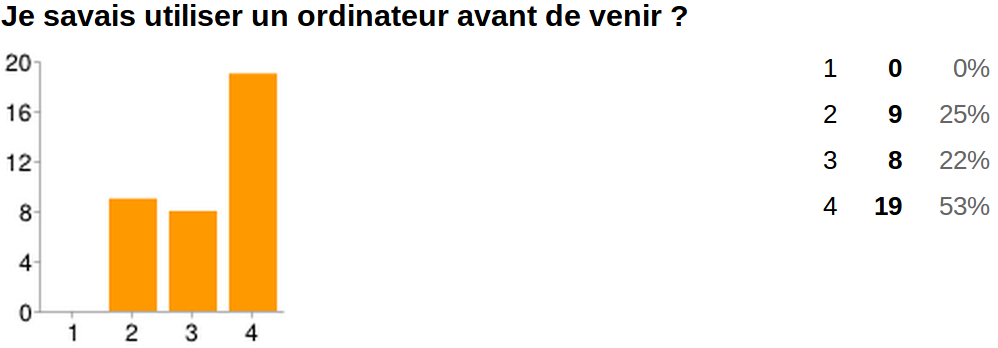
\includegraphics[scale=0.3]{content/8-validation/images/avant}
    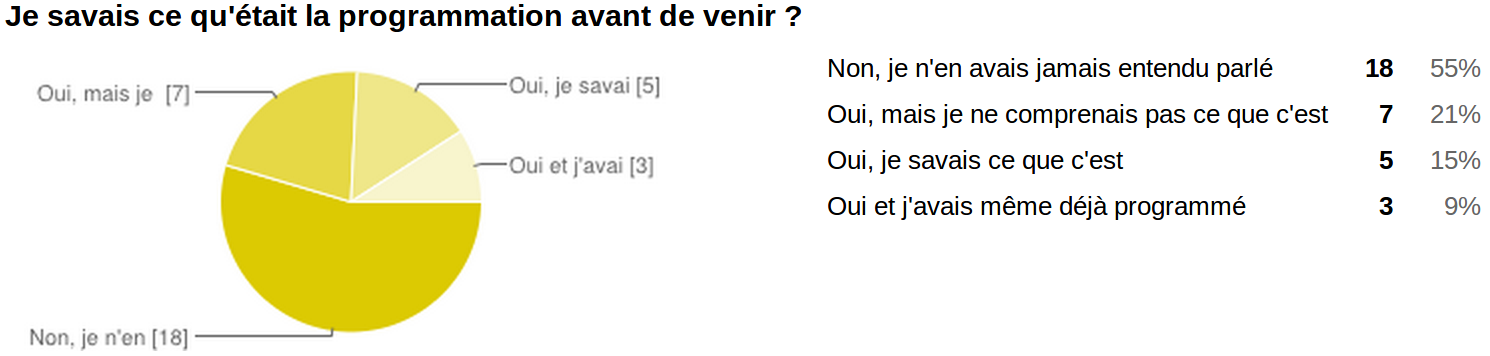
\includegraphics[scale=0.2]{content/8-validation/images/programmation}
    \caption{Auto estimation du niveau en informatique et en programmation des participants avant l'activité}
    \label{fig:niveau-avant}
  \end{center}
\end{figure}
\begin{figure}[ht]
  \begin{center}
    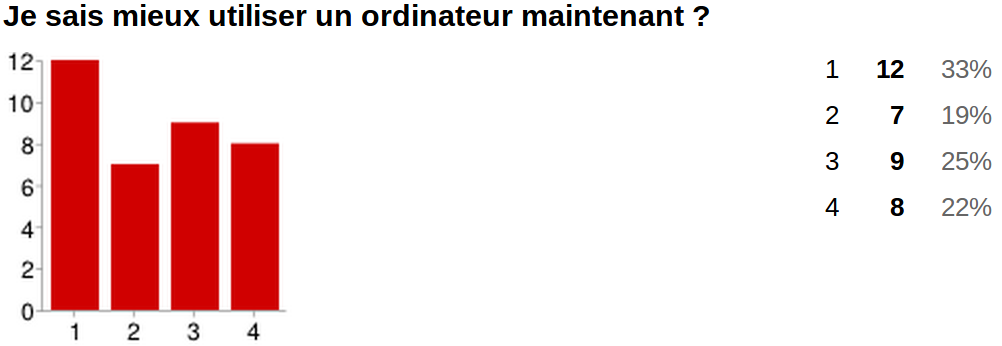
\includegraphics[scale=0.3]{content/8-validation/images/apres}
    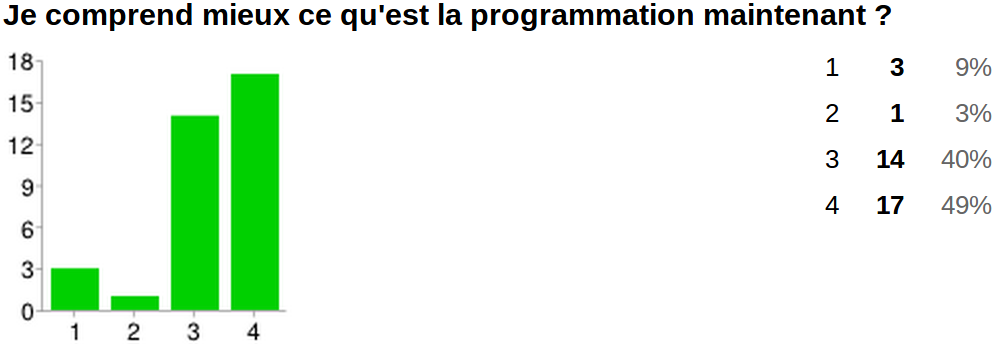
\includegraphics[scale=0.3]{content/8-validation/images/apres-programmation}
    \caption{Auto estimation du niveau en informatique et en programmation des participants après l'activité}
    \label{fig:niveau-apres}
  \end{center}
\end{figure}

\paragraph{Appréciation des missions}
\label{appreciation}
Au delà de l'évaluation de leur niveau, ils ont également dû évaluer séparément chaque mission. Les graphiques représentant cette évaluation sont sur la figure \ref{fig:evaluation-mission}. On voit que les missions qui ont été le moins appréciée sont la troisième, soyons courtois, et la quatrième, chien et chat. La notation de la quatrième mission peut largement s'expliquer par la frustration qu'ils ont eu de ne pas avoir le temps de finir la mission. Pour la troisième, les retours indiquait qu'ils avait trouvé cette mission trop simple. Il faudrait repenser cette mission en y intégrant le déplacement du personnage par exemple.\\


\begin{figure}[ht]
  \begin{center}
    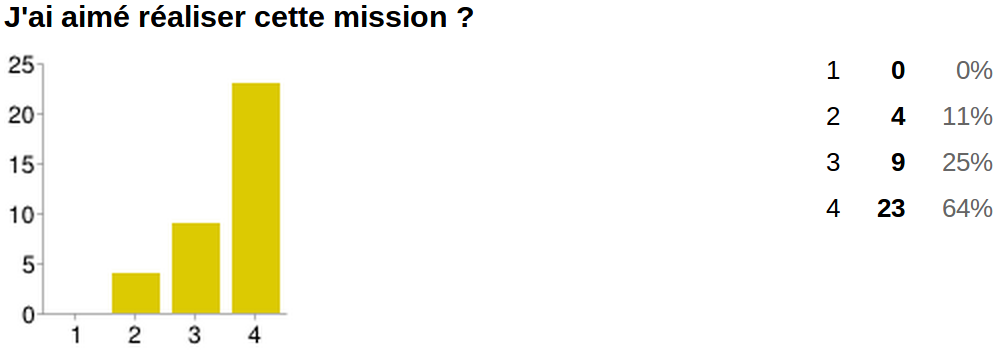
\includegraphics[scale=0.3]{content/8-validation/images/voiture}
    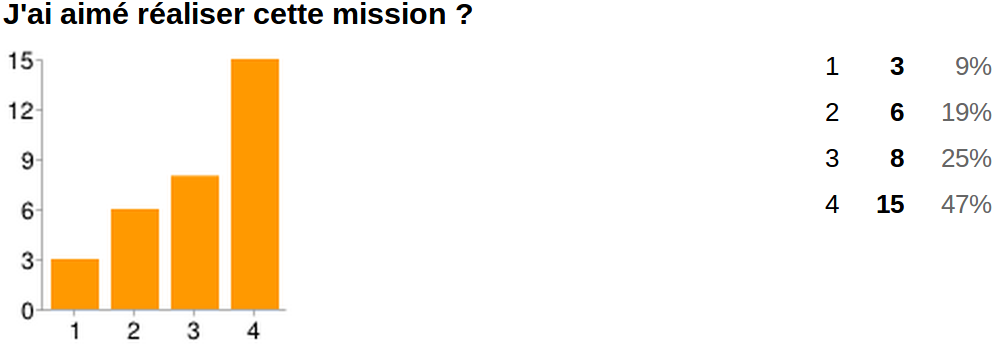
\includegraphics[scale=0.3]{content/8-validation/images/helico}
    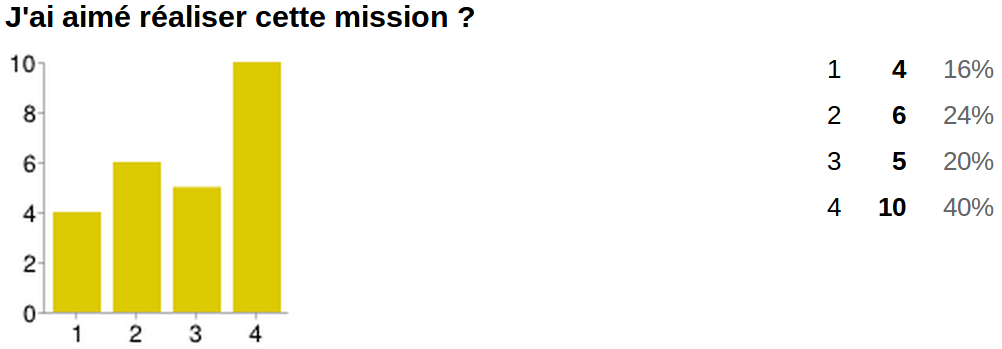
\includegraphics[scale=0.3]{content/8-validation/images/courtois}
    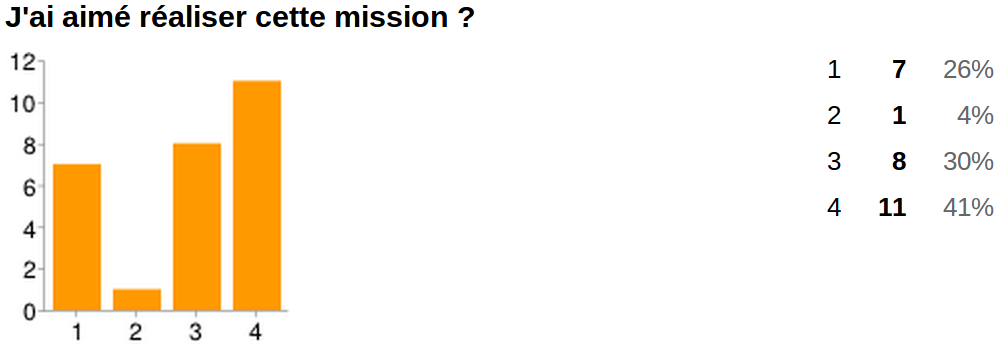
\includegraphics[scale=0.3]{content/8-validation/images/chien}
    \caption{Évaluation des missions par les enfants: En voiture \ref{mission-voiture}, hélicoptère \ref{mission-helicoptere}, soyons courtois \ref{mission-courtois}, tu ne m'attrapera jamais \ref{chien-chat}}
    \label{fig:evaluation-mission}
  \end{center}
\end{figure}

\paragraph{Appréciation des professeurs}
A propos des retours fait par les professeurs, ils sont en annexe \ref{result-prof}. Les retours étaient très positif et les professeurs d'humanité étaient intéresser par l'application pour l'utiliser dans leurs cours.

\paragraph{Analyse des missions}
La première missions a été la plus laborieuse ce qui était prévu. Cependant cette mission a le plus haut taux d'appréciation des enfants et donc en plus de remplir sa mission, elle est bien appréciée par ces dernier.\\

La seconde mission, celle de l'hélicoptère, a été appréciée mais comme cité plus haut \ref{analyse-scienceinfuse}, elle pourrait être séparé en deux missions. Beaucoup d'étudiants ont eu besoin d'aide pour cumuler ces deux concepts en une fois.\\

La troisième mission, soyons courtois, est la moins apprécié car trop facile. Une piste comme suggéré plus haut \ref{appreciation}, serait de rajouter l'implémentation des mouvements à cette mission.\\

La quatrième mission, chien et chat, a passionné les élèves mais ils ont été frustrés par le manque de temps. Personne n'a réussi à la finir. Il faudrait peut être plus guider les étudiant dans cette mission. Par exemple, tout les blocs étaient accessible pour cette mission dans l'optique qu'ils puissent voir ce qui est possible de faire. A posteriori, ce n'est pas une bonne idée car ils se perdent dans la masse de blocs disponibles.

\paragraph{Tranche d'âge}
Un objectif de ce travail est que les enfants puissent utiliser cette application de manière quasi autonome. Dans ce sens, les expériences ont montré que les enfants de début d'humanité sont plus aptes à travailler de manière autonome que les élèves de primaire.
Pour utiliser l'application avec des élèves de primaire, il faudra soit une plus grande maîtrise de la par du professeur soit plus d'encadrant.

% Les grands vont plus vite

% mission voiture cool pour la structuration
% débouché sur du concret

% différence d'age
% appréciation des missions



chiffre et analyse de notre formulaire prof et student.













